%XeTeX
\documentclass[a4paper, 11pt, titlepage]{report}

%Font stuff
\usepackage{fontspec}
\setmainfont[Ligatures={TeX}]{Adobe Caslon Pro}
%1.5 line spacing
\usepackage{setspace}
\onehalfspacing
%\renewcommand{\baselinestretch}{1.2}

%New line between paragraphs, not indentation
\usepackage[parfill]{parskip}

%Make it look good
\usepackage{microtype}
%Colours
\usepackage{xcolor}
\definecolor{brown}{HTML}{85661E}
\definecolor{maroon}{HTML}{800B0B}
\definecolor{navyblue}{HTML}{1E5A9C}

%Margins
\usepackage[top=2.2cm, bottom=2.2cm, left=2.5cm, right=2.5cm]{geometry}

%For appendix
\usepackage[titletoc, title]{appendix}
%Maths
\usepackage{mathtools}
%\usepackage{xfrac} %For sfrac
\usepackage{unicode-math}
 %Use XITS for the TOC as LMM causes hyperref to make buggy click boxes
%\setmathfont{xits-math.otf}
%Footnotes at the bottom
\usepackage[bottom]{footmisc}

%PDF hyperlinks
\usepackage{hyperref}
\hypersetup{
     colorlinks		= true,
     citecolor		= maroon,
     linkcolor		= maroon,
     urlcolor		= navyblue,
     bookmarksopen	= false,
     pdfpagemode	= UseNone,
     pdftitle		= {CITS3001 Assignment Report - 2014},
     pdfauthor		= {Jeremy Tan, 20933708},
     pdfsubject	= {Assignment 2014 - Threes}
}

%Tables
\usepackage{float}
\usepackage{caption}
\captionsetup[table]{skip=7pt}

%Headings
\usepackage{fancyhdr}
\pagestyle{fancy}
\addtolength{\headheight}{2.5pt}
\renewcommand{\chaptermark}[1]{\markboth{\thechapter~~#1}{}}
\renewcommand{\sectionmark}[1]{\markright{\thesection~~#1}{}}
\lhead{\bfseries \leftmark}
\rhead{\bfseries \thepage}
\cfoot{}

%Chapter marks
\usepackage[compact]{titlesec}
\titlespacing*{\chapter}{0pt}{-50pt}{0pt}
\titleformat{\chapter}
	{\normalfont\LARGE\bfseries}{\thechapter.}{0.8em}{}
	
%Importing files
\usepackage{import}
\usepackage{pgf}
\usepackage{tikz}
%\usepackage{lipsum}

% Sub/Superscripting
\newcommand{\ts}{\textsuperscript}
\newcommand{\tu}{\textsubscript}

%Code
\usepackage{listings}
\usepackage{accsupp}% http://ctan.org/pkg/accsupp
\newcommand{\emptyaccsupp}[1]{\BeginAccSupp{ActualText={}}#1\EndAccSupp{}}
\usepackage{xcolor}
\definecolor{mygreen}{rgb}{0,0.6,0}
\definecolor{mygray}{rgb}{0.5,0.5,0.5}
\definecolor{mymauve}{rgb}{0.58,0,0.82}
\lstset{
  basicstyle=\ttfamily\footnotesize\footnotesize,        % the size of the fonts that are used for the code
  breakatwhitespace=false,         % sets if automatic breaks should only happen at whitespace
  breaklines=true,                 % sets automatic line breaking
  captionpos=b,                    % sets the caption-position to bottom
  commentstyle=\color{mygreen},    % comment style
  deletekeywords={...},            % if you want to delete keywords from the given language
  escapeinside={\%*}{*)},          % if you want to add LaTeX within your code
  extendedchars=true,              % lets you use non-ASCII characters; for 8-bits encodings only, does not work with UTF-8
  frame=single,                    % adds a frame around the code
  columns=true,
  keepspaces=true,                 % keeps spaces in text, useful for keeping indentation of code (possibly needs columns=flexible)
  keywordstyle=\color{blue},       % keyword style
  morekeywords={*,...},            % if you want to add more keywords to the set
  numbers=left,                    % where to put the line-numbers; possible values are (none, left, right)
  numbersep=5pt,                   % how far the line-numbers are from the code
  numberstyle=\tiny\color{mygray}\emptyaccsupp, % the style that is used for the line-numbers
  rulecolor=\color{black},         % if not set, the frame-color may be changed on line-breaks within not-black text (e.g. comments (green here))
  showspaces=false,                % show spaces everywhere adding particular underscores; it overrides 'showstringspaces'
  showstringspaces=false,          % underline spaces within strings only
  showtabs=false,                  % show tabs within strings adding particular underscores
  stepnumber=1,                    % the step between two line-numbers. If it's 1, each line will be numbered
  stringstyle=\color{mymauve},     % string literal style
  tabsize=2,                       % sets default tabsize to 2 spaces
  %title=\lstname                   % show the filename of files included with \lstinputlisting; also try caption instead of title
}

%Because typing it is a pain
\newcommand{\threes}{\emph{Threes!}}

\begin{document}
\begin{titlepage}
	\title{CITS3001 -- Algorithms \& Artificial Intelligence\\Assignment Report -- Threes}
	\author{
\includegraphics[width=150pt]{figures/uwacrest.pdf}\\[2em]
		Jeremy Tan, 20933708 }
	\date{May 2014}
	\maketitle
	\centering
\end{titlepage}

\chapter{Problem overview}
\begin{figure}[H]
	\centering
	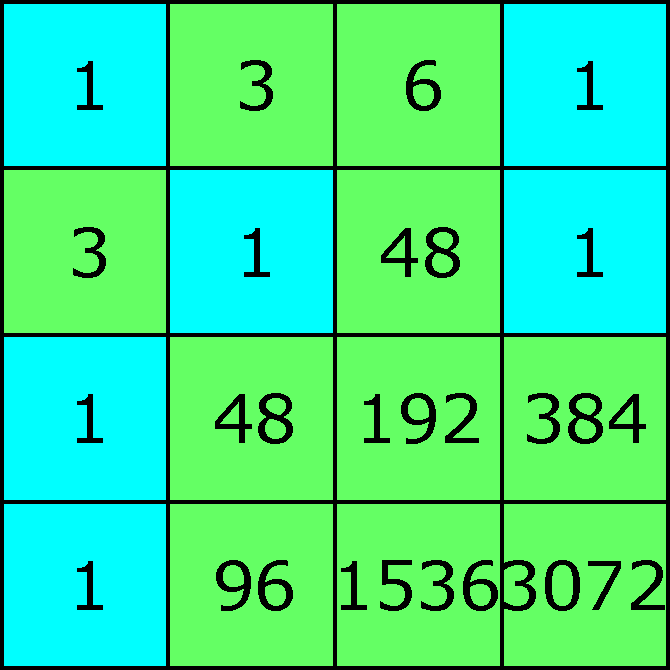
\includegraphics[width=0.35\textwidth]{figures/endboard.pdf}
	\caption{An example end-state board of \threes{}.}
\end{figure}

\threes{}\cite{threes} is a simple puzzle game involving a 4x4 grid, where the objective is to `slide' the tiles on the board such as to maximise the score according to a set of rules. This game was the basis of this project, being to develop a program that could play a modified version of \threes{} at a rate of 5-10 moves per second.

While largely the same, rules concerning the placement of tiles and which tiles would be inserted next after each slide were modified, making the game completely deterministic. In particular, the sequence of tiles which would be inserted after every move was known, while the next tile to be inserted was always placed in the row with the lowest lexicographic score, or in the `most clockwise' row for the case of a tie.

\section{Prior work}
With \threes{} being relatively new, the availability of pre-existing solvers was quite limited. Two works were considered: one being a solver for \threes{}\cite{tsolver}, and another being a solver for a derivative game, \emph{2048}\cite{2048solver}. Of interest was that all existing solutions used a minimax strategy with $\alpha$--$\beta$ pruning. As the modified version of \threes{} was deterministic, minimax was not an applicable solution. Of more importance was understanding \emph{how} these solvers distinguished good board states from bad ones.

\subsection{\threes{} solver} \label{threes-solver}
This solution\cite{tsolver} made use of a heuristic that considered the ``friction'' of a board state, which was essentially a measure of how easy it was to combine adjacent tiles. Boards which could freely combine adjacent tiles received a lower ``friction'' compared to those where adjacent tiles were not combinable. The goal was therefore to go for the board with the lower ``friction''.

Although this heuristic was not directly considered, it was found that in coming up with other heuristics, they followed a similar train of thought --- to maximise the number of combinable tiles on the board at any one time.

\subsection{2048-AI}\label{2048-solver}
While the game of \emph{2048} is not the same as \threes{}, it was derived from it, which was why this was considered. It was found that the similarity did lead to the discovery of some quite good heuristics that were also applicable to this game. Multiple heuristics were used, including:
\begin{enumerate}
	\item{The number of empty tiles present}
	\item{The ``smoothness'' of the board}
	\item{The ``monotonicity'' of the board}
	\item{The maximum value on the board}
\end{enumerate}

The author described in detail why such heuristics were used\cite{2048explanation}. Overall, it was found that the first two were particularly useful, while the latter two could not be successfully used. 

It was found that maximising the number of empty tiles was perhaps one of the most important characteristics of defining a ``good'' board. This was because having more free tiles allows for significantly greater freedom and flexibility when accommodating for new tiles. Implicitly, this heuristic has the effect of encouraging tiles to be combined where possible, in order to maximise the number of free tiles.

The second useful heuristic of ``smoothness'' was also important, but to a somewhat lesser extent. ``Smoothness'' is a measure of how different adjacent tiles are from each other ---  that is, boards where adjacent tiles have a similar value are more smooth than boards where low-valued tiles are adjacent to high-valued tiles. This has the effect of tending to gather similar-valued tiles on the board, making it easier to combine them when needed. It was interesting to note that the particular implementation of ``smoothness'' used in this project tended to gather high valued tiles in the lower right-hand corner of the board.

``Monotonicity'' is a measure of how well tiles increase in value monotonically along any row or column. This helps to prevent a condition known as ``checkerboarding'', where high valued tiles alternate with low valued tiles. Checkerboarding is highly undesirable, as it effectively prevents tiles from being combined, and can quite quickly lead to a premature end-state. Nevertheless, in testing it was found that a heuristic based on monotonicity did not have any significant effect. Instead, a different heuristic involving determining how many times a row or column changes from increasing to decreasing (and vice-versa) value was found to be more effective.

\subsection{Common player strategies}
In final consideration were the common strategies\cite{threes-strategies} players used to maximise the score in \threes{}.

Apart from that already discussed, additional suggestions involved maximising the degrees of freedom (how many directions you can move in), and using the `corner' strategy of keeping large valued tiles in one corner. In general, it was found that the degrees of freedom at any board state did not change from four until you were about to approach a terminal state. This meant that the degrees of freedom was a good measure of when a board state was `bad', and should, if possible, be avoided. 

Although not intentional, the smoothness heuristic used also enforced the `corner strategy', as previously mentioned in section~\ref{2048-solver}.

\section{Potential approaches to solving the modified version of \threes{}}
The fact that the game was made to be deterministic heavily influenced the strategies considered for `solving' the game. In essence, the determinism meant that the complete game tree could theoretically be generated, breaking the problem down into just choosing the path that gave the maximal score. Quite simple and common uninformed search strategies such as a depth-first or breadth-first search could be utilised in this manner, effectively `brute-forcing' the solution.

However, \threes{} has a branching factor of 4, as you can move in up to 4 directions (left, up, right, down). This branching factor makes a complete expansion of the game tree unfeasible, particularly for games where a long sequence of tiles is possible. For example, it is not uncommon to have a game that runs for around 2000 moves. A complete search to that depth would require about 10\ts{1204} nodes to be expanded --- even if they could be expanded at 1ns/node, it would still take 10\ts{1195} seconds, or about 10\ts{1187} years.  

In reality, the absolute maximum lookahead that can be reasonably achieved is to around a depth of 14. Assuming that one board takes 64 bytes (16 x 4 byte unsigned integers), a complete breadth-first search would require 17.18GB, which while feasible with present day consumer-grade hardware, is quite near the limit. 

Informed search strategies, such as A* were also considered to be possible, and would be highly desirable over uninformed search strategies, given that with the right heuristics, a good solution is likely to be found sooner. However, it is debatable whether or not a useful \emph{admissible} heuristic exists for this game. 

For both informed and uninformed search strategies, versions with more restricted memory usage (e.g. IDFS, SMA*, IDA*) could be used to overcome concerns over excessive memory usage.

\chapter{Implementation details}

\chapter{System analysis}

\chapter{Consideration of alternative solutions}

%---------------------------------------------------------
%Referencing
%---------------------------------------------------------
\renewcommand{\bibname}{References}
\bibliography{references/refs}
\bibliographystyle{ieeetr}  
\addcontentsline{toc}{part}{References}
%---------------------------------------------------------

\end{document}